
\section{Routing in Toulouse}

The main aim of our application is to provide a coherent routing tool, enabling people with ASD to cross the city in good conditions, avoiding as far as possible interferences that could cause them discomfort. Before we can apply heuristics to adapt routes to the specific needs of people with ASD, we first need to obtain optimized routes between the desired addresses, then check whether they are suitable for the user and, if necessary, modify them using our heuristics.\newline

In this section, we'll talk more specifically about how we were able to obtain and display real-time journeys in the city of Toulouse by interacting with the APIs provided by Tisséo.\newline

\subsection{Displaying Data}
The first step to making a working routing application was to display a map of the Toulouse city on the application. We had to choose the right libraries and data to have a correct and precise map of Toulouse's streets. We searched for the best tool and found the OpenStreetMap database, an open-source and free-to-use database, which represents a map of the whole world. This database can be used via several libraries, which allows us to easily interact with our map. We set a map with several parameters, to display the map with a correct zoom and at the exact coordinates of Toulouse.\newline


Now that we have a correct map of Toulouse, we can correctly display the routes we want to take. We created another activity so that the user could specify the characteristics of the journey, such as the departure and arrival addresses of the desired trip. The user can also select the desired modes of transport, including metro, bus, walking and cycling, as well as the desired departure time or arrival time.\newline

\begin{center}
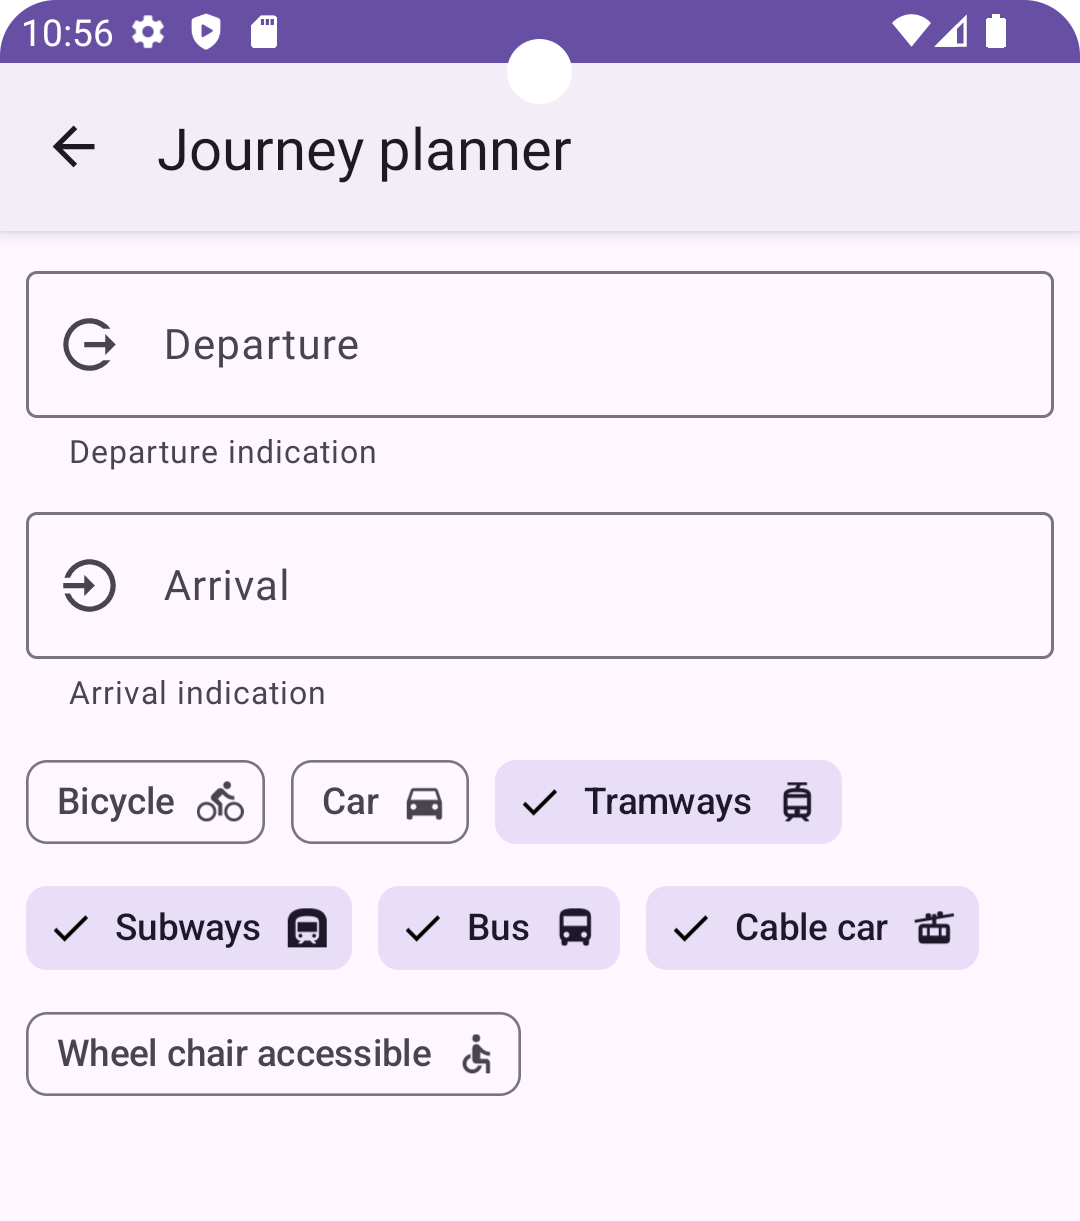
\includegraphics[scale=0.25]{content/journey.png}
\newline
The journey planner page of our application
\newline
\end{center}

The Places API gives us access to Tisséo's vast database of known places in the city of Toulouse. We use this service to ensure that addresses provided by users are validated and recognized in Tisséo's infrastructure and interfaces. This validation process avoids potential errors that could result from the use of unrecognized or ambiguous addresses. It contributes to the accuracy and reliability of our route planning functionality, by returning verified addresses.
In addition, the API offers features such as auto-completion or suggestions. Those features can help users enter addresses more efficiently and accurately. This further enhances the user experience by reducing the likelihood of input errors.\newline

\subsection{Journey Routing}
When the journey search is launched, the application will call the Journey service of the Tisséo API to request one or more journeys between the addresses provided. The Journey API is responsible for retrieving route information between the addresses given by the user, while also taking into account its chosen modes of transportation and the optional departure or arrival dates.\newline

The Journey API processes this request with the user parameters. It returns a response containing several journeys that match the user's needs. This response is formatted in JSON and contains detailed information on each recommended journey. In that information, we can find the route segments to travel across, the time needed to accomplish the journey or the different turns to make. We enable users to access up-to-date and accurate route information, tailored to their specific needs. This enables users to make informed decisions when planning their journeys, whether to work, to explore the city or to find their way around unfamiliar areas.\newline

With the information extracted from the Tisséo API response, we need to reconstruct a route that can be displayed on our map. We use the Road class, a structure provided by the Open Street Map library that allows us to represent a route as a series of GPS coordinate points. The journey is divided into several “steps”. Each step is a part of the journey that uses only one mode of transportation and on which only one action is done. Some examples of what a step is could be “Walk on the Capitole Street for 500m and turn left” or “Take the bus 27 until the bus stop Rangueil”. This structure lets us add the entire route to the map. But at the same time, it grants us the right to add points of interest, to specify additional information about the route, such as where to change streets or transportation mode but also the duration and the length of the next step.\newline

Thanks to our road structure, we can easily add the route to the map. By tapping on the step icons, you can obtain information on the route and the next step.\newline

\begin{center}
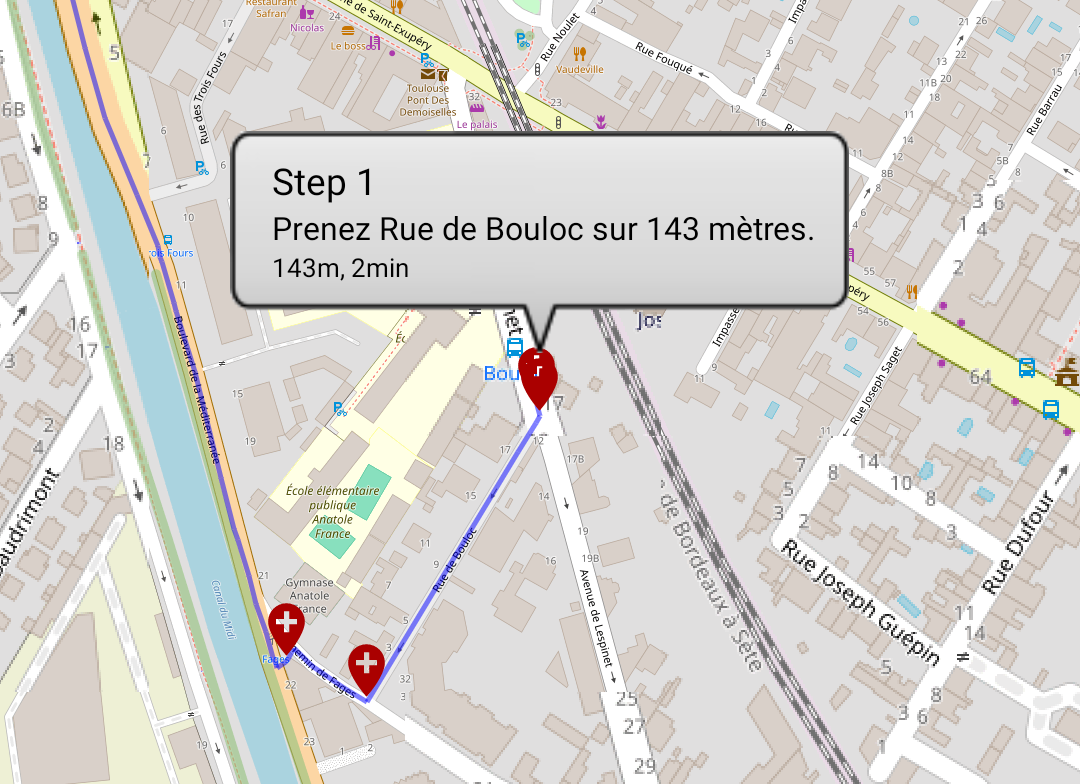
\includegraphics[scale=0.30]{content/step_cut.png} 
\newline
Visualisation of a step
\newline
\end{center}

Our application enables anyone to find their way around Toulouse by public transport, on foot or by bike. The suggested route takes into account real-time events and proposes the best solution according to current conditions.\newline
